\section{Model Capacity and Overfitting}

The capability of a model refers to its \textbf{ability to fit a wide range of functions}. Indeed, it represents the intrinsic complexity of the model and its ability to capture relations in the data. \textit{In other words, it describes how complex is the function it represents.}

Models with low capacity may have difficulty adapting to the training set, while those with high capacity may suffer from overfitting, that is, overfitting to the training data leading to poor generalization to new data.

Model capacity is closely related to the hypothesis space, which represents the set of all features that the model can potentially learn. A model with a higher capacity will have access to a larger hypothesis space, allowing it to learn more complicated relationships in the data.

\begin{figure}[!htbp]
    \centering
    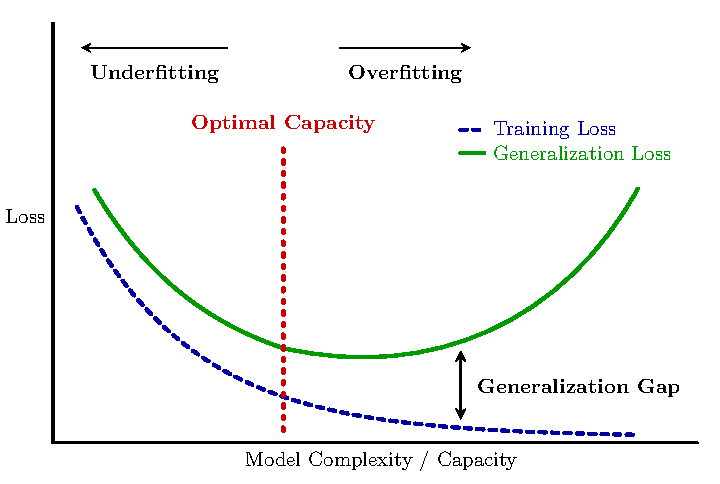
\includegraphics[width = \linewidth]{tikz/chapter4 - Model Capacity.pdf}
    \caption{Complexity of a Model with respect to the Losses}
\end{figure}

In the figure above, it is evident that as the complexity of the model increases, the loss on the training set tends to decrease, while the loss on generalization (e.g., on the test set) may increase, causing a gap between the losses known as the \textbf{generalization gap}.

To deal with overfitting, it is important to choose a model with the right capacity. This means setting the capacity so that it is high enough to capture the main regularities in the training data, but not so high that it also captures spurious regularities or noise in the data. \textit{Basically, it is a matter of finding a balance between the complexity of the model and its capacity for generalization.}

In addition to controlling model capacity, there are other strategies to reduce overfitting. For example, \textbf{collecting more training data} can help the model better capture the variety of relationships in the data. Alternatively, \textbf{ensembling techniques}, such as averaging many different models (e.g. bagging), can be used. These strategies help avoid overfitting to training data, allowing the model to generalize better to new data.

\textit{Are there alternatives to cope with overfitting? Yes, regularization techniques! These provide effective tools for optimizing model performance. In the next sections, we will dive into the details of these powerful assets!}

To give you a taste, here is an overview of the various regularization strategies we will see:

\begin{figure}[!htbp]
    \centering
    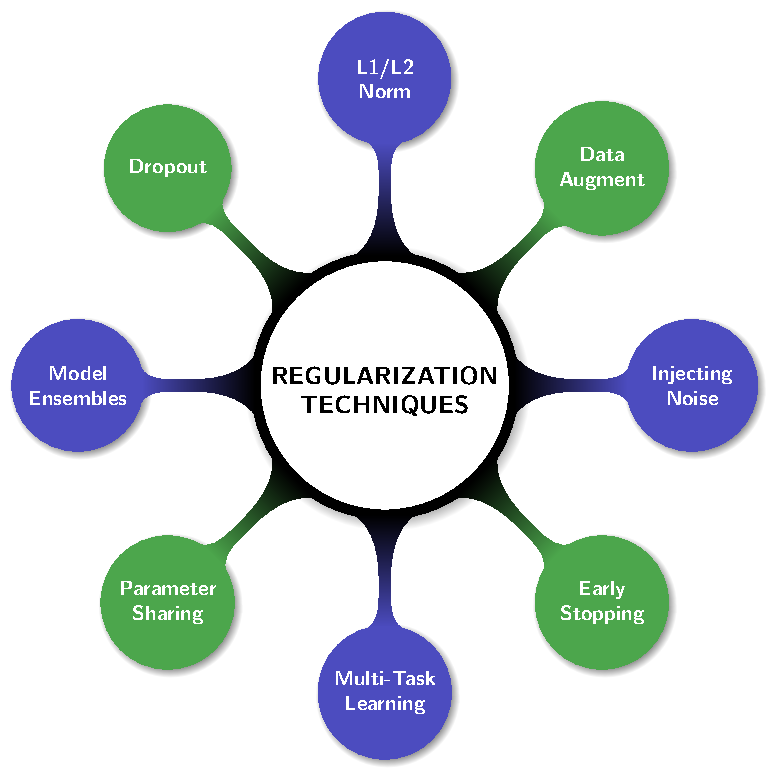
\includegraphics[width = 0.8\linewidth]{tikz/chapter4 - Regularization Schema.pdf}
    \caption{Different Regularization Strategies}
\end{figure}

\section{Parameter Norm Penalties}

We start with this first type of normalization in which we add a penalty to the loss function during training, which then \textbf{affects the size of the weights (parameters)} of the model. Here is the general formula for the error function:

$$
\tilde{L}(\mathbf{W}) = L(\mathbf{W}) + \lambda \Omega(\mathbf{W})
$$

The \textbf{\textcolor{myred}{Regularization L2}}, also known as \textbf{\textcolor{myred}{Ridge}}, adds a term to the loss function proportional to the \textbf{\textcolor{myred}{square norm of model weights}}. Mathematically, the formula for L2 regularization is given by:

$$
\Omega(\mathbf{W}) = \frac{1}{2} \sum_{l} ||\mathbf{w}_l||^2
$$

This is inserted into the error function, obtaining the regularized loss function $\tilde{L}(\mathbf{w})$:

$$
\tilde{L}(\mathbf{W}) = \sum_{i=1}^{n} L(f(x_i, \mathbf{W}), y_i) + \textcolor{myred}{\frac{\lambda}{2} \sum_{l} ||\mathbf{w}_l||^2}
$$

Where:
\begin{itemize}
    \item $\sum_{i=1}^{n} L(f(x_i, \mathbf{W}), y_i)$ represents the sum of losses on all training data $(x_i, y_i)$.
    \item $\frac{\lambda}{2} \sum_{l} ||\mathbf{w}_l||^2$ represents the L2 regularization term, where $|\mathbf{w}_l||^2$ is the squared norm of the model weights and $\lambda$ is the regularization parameter.
    \item The sum over $l$ represents the sum over all the weights of the model.
\end{itemize}

$\lambda$ is \textbf{the hyperparameter that controls the importance of regularization}, i.e., it determines how much weight to give to the penalty of the model weights with respect to performance on the training data.

The use of L2 regularization leads the model weights to \textbf{tend to smaller values}, thus avoiding extremely high values that could lead to overfitting. In addition, this technique promotes the creation of simpler models.

On the other hand, the \textbf{\textcolor{mygreen!90!black}{Regularization L1}}, also known as the \textbf{\textcolor{mygreen!90!black}{Lasso}}, adds a term to the loss function proportional to the \textbf{\textcolor{mygreen!90!black}{absolute norm of model weights}}. The L1 regularization formula is expressed as:

$$
\Omega(\mathbf{W}) = \sum_{l} |\mathbf{w}_l|
$$

Again, we insert in the loss function:

$$
\tilde{L}(\mathbf{W}) = \sum_{i=1}^{n} L(f(x_i, \mathbf{W}), y_i) + \textcolor{mygreen!90!black}{\lambda \sum_{l} |\mathbf{w}_l|}
$$

Where:
\begin{itemize}
    \item $\sum_{i=1}^{n} L(f(x_i, \mathbf{W}), y_i)$ represents the sum of losses on all training data $(x_i, y_i)$.
    \item $\lambda \sum_{l} |\mathbf{w}_l|$ represents the L1 regularization term, where $|\mathbf{w}_l|$ is the absolute norm of the model weights and $\lambda$ is the regularization parameter.
    \item The sum over $l$ represents the sum over all the weights of the model.
\end{itemize}

Unlike L2 regularization, L1 regularization favors \textbf{sparsity of weights}, that is, many weights tend to become exactly zero. This behavior is also useful for feature selection, since it makes the features most relevant to the model more obvious.

To summarize, here is a figure that visually shows how L1 and L2 regularization affect model weights differently:

\begin{figure}[!htbp]
    \centering
    \includegraphics[width = \linewidth]{tikz/chapter4 - L1 and L2 plot.pdf}
    \caption{L2 Regularization and L1 Regularization Plots}
\end{figure}


The plot represents the space of model weights/parameters.

In the center of the gradient error is the point where the model error is lowest. At this point, the model shows the best performance on the training data.

Next, you will notice an overlap between the gradient error and the gradient of the L1 or L2 norm penalty. This is an optimization point where the overall model error is minimized, also taking into account the regularization penalty. Here the \textbf{right balance between error reduction and model complexity} is achieved, thus avoiding both underfitting and overfitting.

For \textbf{\textcolor{mygreen}{L1 regularization}}, it will be observed that many of the weights in the model will touch the L1 Norm function in the zero abscissa, representing null weights. This indicates that L1 regularization \textbf{favors sparsity of the weights}.

For \textbf{\textcolor{myred}{L2 regularization}}, you will notice a gradual reduction of the weights, but none will be exactly zero. This represents that L2 regularization acts more uniformly, \textbf{reducing the magnitude of the weights without completely zeroing them}.

\section{Data Augmentation}

One of the main challenges in training models is the availability of sufficient and diverse training data. Data augmentation is a strategy that aims to improve model generalization by \textbf{increasing the amount and variety of training data}. The idea behind it is that the more training data we have, the better the model can learn to generalize to new data not seen during training.

Data augmentation is particularly effective in classification tasks, where it is relatively easy to generate new samples by transforming existing ones. This approach is based on the fact that the \textbf{main task of the classifier is to be invariant to a wide range of transformations of the input data}. For example, in the case of images, we can generate new samples by applying transformations such as rotation, translation, color change, scaling, and so on. The goal is to create a diversity of samples that cover as much of the input data space as possible, thus helping the model learn a more robust and general representation of discriminative features.
    
Some problems may require special precautions during data augmentation. For example, in the context of character recognition using datasets such as MNIST, it is important not to apply transformations that would change the class, such as transformations that might turn a '6' into a '9'.
    
Data augmentation can also be applied to different types of data, such as \textbf{acoustic and textual data}. For example, for acoustic data, transformations such as pitch shift, stretching time and dynamic range compression can be applied. For textual data, one can use techniques such as substitution, deletion, and letter insertion, or use synonyms and modify adjectives.

\section{Injecting Noise}

Gaussian noise as input can be used as a regularizer in neural models. Specifically, each component of the input \( x_i \) can be modified by adding Gaussian noise \( \mathcal{N}(0, \sigma_i^2) \), so the equation becomes:

$$ x_i = x_i + \textcolor{mybluee}{\mathcal{N}(0, \sigma_i^2)} $$

As for the output \( y_j \) of a layer, it can be expressed as the sum of the original output and the Gaussian noise \textbf{amplified by the weight squared}, so the equation becomes:

$$ y_j = y_j + \textcolor{mybluee}{\mathcal{N}(0, w_i^2 \sigma_i^2)} $$

where \( N(0, \sigma_i^2) \) represents Gaussian noise with zero mean and variance \( \sigma_i^2 \), \( w_i \) represents the weight associated with the input \( x_i \).

This contributes additively to the quadratic error, causing the model to minimize the overall error, which then \textbf{tends to minimize the square weights as well}. This effect is similar to L2 regularization through noisy inputs. 

\textbf{High levels of noise generate a smoother function}. This is useful in applications where a smooth function is preferred.

In \textbf{autoencoder models for denoising}, noise injection is a common practice. The goal is to teach the neural network to reconstruct the original input from the noisy input. This technique is often used in unsupervised learning algorithms.

\textit{But can noise only be added to inputs? Absolutely not! It can also be added to weights and labels in neural models!} Adding noise to the inputs makes the learned function smoother, while \textbf{adding noise to the weights encourages the network to be more robust to random variations in the training data} (we get a kind of "flexibility" in the model's weights). This can be especially useful when the model is in regions of the weight space where variations in individual weights do not significantly affect the model output. \textbf{Adding noise to labels can discourage overconfident model behavior}, such as during cross-entropy loss learning, thus preventing overestimation of class probabilities (cross-entropy assigns very large values for the correct class and very small values for the wrong classes). A common practice in this case is the application of "\textbf{label smoothing}", which is the random modification of labels.

\section{Early Stopping}

Early Stopping is a technique used in model training to prevent the model from becoming too specialized on the training data. 
This technique is based on the idea of monitoring the performance of the model on a validation dataset during training and \textbf{stopping training when the performance on the validation set starts to deteriorate, even if the performance on the training set continues to improve}.

The number of training steps is seen as another \textbf{hyperparameter that needs to be optimized}. The Early Stopping procedure can be summarized in the following steps: It starts with small initial weights. Each time the error on the validation set improves, you keep a copy of the model parameters. When training ends, you return the parameters \textbf{for which the validation error is smallest}.

However, it is \textbf{important to select the stopping point correctly}, since an early stopping point could prevent the model from learning important information, while stopping too late could lead to overfitting. Consequently, the number of epochs or iterations before stopping must be carefully selected during the training phase.

\section{Multi-Task Learning}

Multi-Task Learning is a learning technique where the model is trained to do \textbf{more than one task at the same time}. For example, we might want to train a model to recognize objects in an image and simultaneously identify their location. This means that the model learns to perform more than one "task" during the same training process.

In Multi-Task Learning, several tasks \textbf{share the same set of input data and some intermediate layers of the neural network}, but may have \textbf{separate final layers for each task}. In this case, the parameters can be of two types: \textbf{task-specific} or \textbf{generic} (shared among all tasks). The former are designed to perform a specific task and learn only from data related to that task (typically found in the upper layers of the network), while the latter are shared across all tasks and can benefit from the combined data of all tasks (typically found in the lower layer of the network).

\begin{figure}[!htbp]
    \centering
    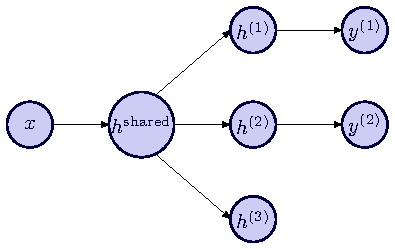
\includegraphics[width = 0.6\linewidth]{tikz/chapter4 - Multi Task Learning.pdf} 
    \caption{Visualization of Multi-Task Learning}
\end{figure}

Multi-Task Learning often compares with self-supervised learning. While in Multi-Task Learning multiple tasks are taught at the same time, \textbf{in self-supervised learning the model learns to represent data in such a way that some information is "hidden"} and must be predicted. For example, it might train a model to predict missing parts of a picture.

In Multi-Task Learning, it is possible to apply \textbf{soft constraints on model parameters}. This means that we can enforce some parameters to be similar to others (this is called \textbf{"Paramaters Tying"}). For example, if we have multiple models performing the same type of classification but with slightly different data, we can force the parameters to be similar to ensure consistency across models.

\section{Parameters Sharing}
\label{c4:parameterSharing}
Parameter Sharing is a technique used in neural networks to enforce that \textbf{certain parameters within the network are exactly the same}. This is done for several reasons, including reducing model complexity and sharing relevant information between different parts of the network.

Sharing parameters within the network offers an advantage over "Paramaters Tying", since only a subset of the parameters need to be stored in memory.

In convolutional neural networks (CNNs), used primarily in computer vision, parameter sharing is a key feature. This is based on two main properties of CNNs:

\begin{itemize}
    \item \textbf{Local Connectivity}: Neurons in one layer are \textbf{connected to only a small region of the previous layer}. This feature allows CNNs to capture local image features.
    \item \textbf{Weight Sharing between Spatial Positions}: This feature allows CNNs to learn displacement-invariant filter kernels, reducing the number of parameters needed and ensuring that the model is \textbf{able to recognize the same features in different parts of the image}. For example, a picture of a cat remains a picture of a cat even if it is shifted by some pixel. 
\end{itemize}

\section{Model Ensembles}

In this technique, instead of relying on a single model, we train several models separately and then have all the models vote on the output for the test examples. The idea behind it is that \textbf{different models will usually make different errors on the test set}. Therefore, by combining the predictions of multiple models, a better overall result can be obtained. \textit{This technique is similar to consulting multiple experts to get more reliable advice.}

One of the most common methods of implementing Model Ensembles is \textbf{Bagging} (Bootstrap Aggregating). In Bagging, several instances of the same model type are trained on \textbf{random subsets of the training set (with replacement)} and then the \textbf{predictions of all models are combined}. 

However, this method requires more computational resources and can be more complex to implement and manage than a single model.

\section{Dropout}

The basic idea of Dropout is to \textbf{randomly turn off some neurons} during the forward pass of the network. This process is \textbf{stochastic}, since the choice of neurons to be eliminated is random. By forcing the network to work with redundant representations, Dropout prevents hidden neurons from fitting too closely to each other and \textbf{forces them to focus on extracting more useful features} for the task.

Dropout can be viewed as training a large set of models, each of which shares network parameters. Each binary Dropout mask leads to a different model, and for each example, the network is trained using a different Dropout mask. \textit{Each value in the mask represents whether the corresponding neuron is active (1) or deactivated (0) during the forward pass of the network.}

Dropout is similar to Bagging, but is more practical. Whereas in Bagging one defines \( k \) different models and builds \( k \) different datasets by sampling from the dataset with replacement, \textbf{Dropout aims to approximate this process with exponentially large numbers of neural networks}.

\begin{figure}[!htbp]
    \centering
    \includegraphics[width = \linewidth]{tikz/chapter4 - Dropout.pdf}
    \caption{Visualization of the Dropout Technique}
\end{figure}

During training, at each step, a binary Dropout mask with a certain inclusion probability is randomly extracted for each neuron. This mask is then used to deactivate some neurons during the forward transition of the network. During testing, ideally we would like to integrate all probability contributions for all masks, but this is \textbf{computationally expensive}. Therefore, we use a \textbf{Monte Carlo approximation}, performing many forward steps with different Dropout masks and averaging all predictions. It has been shown that this procedure is equivalent to taking the average of all possible neural networks.

